\documentclass[12pt,a4paper]{article}\usepackage[]{graphicx}\usepackage[]{color}
% maxwidth is the original width if it is less than linewidth
% otherwise use linewidth (to make sure the graphics do not exceed the margin)
\makeatletter
\def\maxwidth{ %
  \ifdim\Gin@nat@width>\linewidth
    \linewidth
  \else
    \Gin@nat@width
  \fi
}
\makeatother

\definecolor{fgcolor}{rgb}{0.345, 0.345, 0.345}
\newcommand{\hlnum}[1]{\textcolor[rgb]{0.686,0.059,0.569}{#1}}%
\newcommand{\hlstr}[1]{\textcolor[rgb]{0.192,0.494,0.8}{#1}}%
\newcommand{\hlcom}[1]{\textcolor[rgb]{0.678,0.584,0.686}{\textit{#1}}}%
\newcommand{\hlopt}[1]{\textcolor[rgb]{0,0,0}{#1}}%
\newcommand{\hlstd}[1]{\textcolor[rgb]{0.345,0.345,0.345}{#1}}%
\newcommand{\hlkwa}[1]{\textcolor[rgb]{0.161,0.373,0.58}{\textbf{#1}}}%
\newcommand{\hlkwb}[1]{\textcolor[rgb]{0.69,0.353,0.396}{#1}}%
\newcommand{\hlkwc}[1]{\textcolor[rgb]{0.333,0.667,0.333}{#1}}%
\newcommand{\hlkwd}[1]{\textcolor[rgb]{0.737,0.353,0.396}{\textbf{#1}}}%
\let\hlipl\hlkwb

\usepackage{framed}
\makeatletter
\newenvironment{kframe}{%
 \def\at@end@of@kframe{}%
 \ifinner\ifhmode%
  \def\at@end@of@kframe{\end{minipage}}%
  \begin{minipage}{\columnwidth}%
 \fi\fi%
 \def\FrameCommand##1{\hskip\@totalleftmargin \hskip-\fboxsep
 \colorbox{shadecolor}{##1}\hskip-\fboxsep
     % There is no \\@totalrightmargin, so:
     \hskip-\linewidth \hskip-\@totalleftmargin \hskip\columnwidth}%
 \MakeFramed {\advance\hsize-\width
   \@totalleftmargin\z@ \linewidth\hsize
   \@setminipage}}%
 {\par\unskip\endMakeFramed%
 \at@end@of@kframe}
\makeatother

\definecolor{shadecolor}{rgb}{.97, .97, .97}
\definecolor{messagecolor}{rgb}{0, 0, 0}
\definecolor{warningcolor}{rgb}{1, 0, 1}
\definecolor{errorcolor}{rgb}{1, 0, 0}
\newenvironment{knitrout}{}{} % an empty environment to be redefined in TeX

\usepackage{alltt}
\usepackage[utf8]{inputenc}
\setlength{\paperheight}{11.7in} % set dimension of \paperwidth to 25 cm
\setlength{\paperwidth}{8.27in}
%%\addtolength{\paperheight}{2in} % enlarge \paperheight by 1 inch
\usepackage[portuguese]{babel}
\usepackage{longtable,booktabs}
\usepackage[T1]{fontenc}
\usepackage{amsmath}
\usepackage{indentfirst}
\usepackage{color}
\usepackage{caption}
\usepackage{amsfonts}
\usepackage{float}
\usepackage[dvipsnames]{xcolor}
\usepackage{amssymb}
\usepackage{graphicx}
\usepackage{lmodern}
\usepackage{subfigure}
\usepackage{caption}
\captionsetup{font=small}% \captionsetup{font=footnotesize}
\usepackage[left=1.5cm, right = 2cm, top=3cm,bottom=2.6cm]{geometry}
\fontsize{12pt}{10cm}\selectfont
\title{Análise descritiva e preditiva sobre \\ segmentação dos clientes Duas Rodas}
\usepackage{float}
\usepackage{fancyhdr}
%% SET DEFAULT FONTFD  
\usepackage{mathptmx}
\usepackage[T1]{fontenc}
%% \usepackage[T1]{fontenc}
%% \usepackage{times}
%% \usepackage{PTSerifCaption} 
%% \usepackage[T1]{fontenc}

\pagestyle{fancy}
\fancyhf{}
\fancyhead[LE,RO]{Mobills Labs}
\fancyhead[RE,LO]{{\small\scshape Relatório de Análise descritiva}}
\fancyfoot[CE,CO]{{\small\leftmark}}
\fancyfoot[LE,RO]{{\small\thepage}}

\renewcommand{\headrulewidth}{2pt}
\renewcommand{\footrulewidth}{1pt}
\IfFileExists{upquote.sty}{\usepackage{upquote}}{}
\begin{document}


\begin{titlepage}
\begin{center}
\begin{minipage}{5in}
\begin{center}
\hspace{-1cm}

\includegraphics[scale=0.23]{figure/logo.png}
\vspace{3.5cm}\\
{\large \scshape Relatório de Análise Descritiva}\\
\vspace{14cm}
{\hspace{1cm}
{\Large FORTALEZA \\ \hspace{1cm} 2018}}
\end{center}
\thispagestyle{empty}
\end{minipage}
\end{center}
\end{titlepage}

\newpage
\section{Análise das despesas}




\begin{knitrout}\tiny
\definecolor{shadecolor}{rgb}{0.969, 0.969, 0.969}\color{fgcolor}\begin{kframe}
\begin{alltt}
\hlcom{##setwd("projetos/Consulta Mobills/")}
\hlstd{Despesas} \hlkwb{<-} \hlkwd{fread}\hlstd{(}\hlstr{"./data/dadosReceitasUsers/Despesas20190711.csv"}\hlstd{)}
\hlstd{Despesas2018} \hlkwb{<-} \hlkwd{fread}\hlstd{(}\hlstr{"./data/dadosReceitasUsers/Despesas20180107.csv"}\hlstd{)}
\hlstd{Despesas} \hlkwb{<-} \hlkwd{do.call}\hlstd{(}\hlstr{"rbind"}\hlstd{,} \hlkwd{list}\hlstd{(Despesas,Despesas2018))}
\hlstd{Despesas} \hlopt \hlkwd{mutate}\hlstd{(}\hlkwc{ano}\hlstd{= lubridate}\hlopt{::}\hlkwd{year}\hlstd{(DataDespesa))} \hlkwb{->} \hlstd{Despesas}
\end{alltt}
\end{kframe}
\end{knitrout}
As medidas de resumo mostram que claramente há valores inválidos e outliers nos dados.

\begin{knitrout}\tiny
\definecolor{shadecolor}{rgb}{0.969, 0.969, 0.969}\color{fgcolor}\begin{kframe}
\begin{alltt}
\hlstd{Despesas}\hlopt{$}\hlstd{Valor} \hlkwb{<-} \hlkwd{gsub}\hlstd{(}\hlkwc{pattern} \hlstd{=} \hlstr{","}\hlstd{,}\hlkwc{replacement} \hlstd{=} \hlstr{"."}\hlstd{, Despesas}\hlopt{$}\hlstd{Valor)}
\hlstd{Despesas}\hlopt{$}\hlstd{Valor} \hlkwb{<-} \hlkwd{as.numeric}\hlstd{(Despesas}\hlopt{$}\hlstd{Valor)}
\end{alltt}
\end{kframe}
\end{knitrout}
\begin{knitrout}\tiny
\definecolor{shadecolor}{rgb}{0.969, 0.969, 0.969}\color{fgcolor}\begin{kframe}
\begin{alltt}
\hlstd{Despesas} \hlopt
  \hlkwd{select}\hlstd{(ano,Valor)}\hlopt
  \hlkwd{split}\hlstd{(.}\hlopt{$}\hlstd{ano)} \hlopt
  \hlkwd{map}\hlstd{(summary)}
\end{alltt}
\begin{verbatim}
## $`2018`
##       ano           Valor        
##  Min.   :2018   Min.   : -10000  
##  1st Qu.:2018   1st Qu.:      9  
##  Median :2018   Median :     22  
##  Mean   :2018   Mean   :    133  
##  3rd Qu.:2018   3rd Qu.:     60  
##  Max.   :2018   Max.   :6000000  
## 
## $`2019`
##       ano           Valor                 
##  Min.   :2019   Min.   :          -15591  
##  1st Qu.:2019   1st Qu.:              10  
##  Median :2019   Median :              25  
##  Mean   :2019   Mean   :     12899026578  
##  3rd Qu.:2019   3rd Qu.:              69  
##  Max.   :2019   Max.   :9000000000000000
\end{verbatim}
\end{kframe}
\end{knitrout}
Para plotar o Histograma dos Valores gastos(Despesas) vamos limitar a variável `Valor` em até 1000 reais. Tendo em vista que quase a totalidade dos dadados se concentram nesse intervalo.
\begin{knitrout}\tiny
\definecolor{shadecolor}{rgb}{0.969, 0.969, 0.969}\color{fgcolor}\begin{kframe}
\begin{alltt}
\hlstd{Despesas} \hlopt
  \hlkwd{group_by}\hlstd{(UsuarioId,}
           \hlkwc{dia} \hlstd{= lubridate}\hlopt{::}\hlkwd{day}\hlstd{(DataDespesa),}
           \hlkwc{mes} \hlstd{= lubridate}\hlopt{::}\hlkwd{month}\hlstd{(DataDespesa),}
           \hlkwc{ano} \hlstd{= lubridate}\hlopt{::}\hlkwd{year}\hlstd{(DataDespesa))} \hlopt
    \hlkwd{summarise}\hlstd{(}\hlkwc{count} \hlstd{=} \hlkwd{n}\hlstd{(),} \hlkwc{valorSoma}\hlstd{=} \hlkwd{sum}\hlstd{(Valor))} \hlopt
    \hlkwd{arrange}\hlstd{(}\hlkwd{desc}\hlstd{(valorSoma))} \hlkwb{->} \hlstd{desp}



\hlstd{Despesas} \hlopt \hlstd{dplyr}\hlopt{::}\hlkwd{filter}\hlstd{(Valor} \hlopt{>} \hlnum{0} \hlopt{&} \hlstd{Valor} \hlopt{<} \hlnum{1000}\hlstd{)} \hlopt
    \hlkwd{ggplot}\hlstd{(}\hlkwd{aes}\hlstd{(Valor,}\hlkwc{y}\hlstd{=..density..))}\hlopt{+}
    \hlkwd{geom_histogram}\hlstd{(}\hlkwc{fill}\hlstd{=}\hlstr{"white"}\hlstd{,}\hlkwc{alpha}\hlstd{=}\hlnum{0.8}\hlstd{)}\hlopt{+}
    \hlkwd{facet_grid}\hlstd{(}\hlopt{~}\hlstd{ano )}\hlopt{+}\hlstd{temaMobills}\hlopt{+}
        \hlkwd{labs}\hlstd{(}\hlkwc{title}\hlstd{=}\hlstr{"Distribuição das despesas"}\hlstd{)}\hlopt{+}
    \hlkwd{scale_x_continuous}\hlstd{(}\hlkwc{limits}\hlstd{=}\hlkwd{c}\hlstd{(}\hlnum{0}\hlstd{,}\hlnum{1000}\hlstd{))}
\end{alltt}


{\ttfamily\noindent\color{warningcolor}{\#\# Warning: Removed 4 rows containing missing values (geom\_bar).}}\end{kframe}
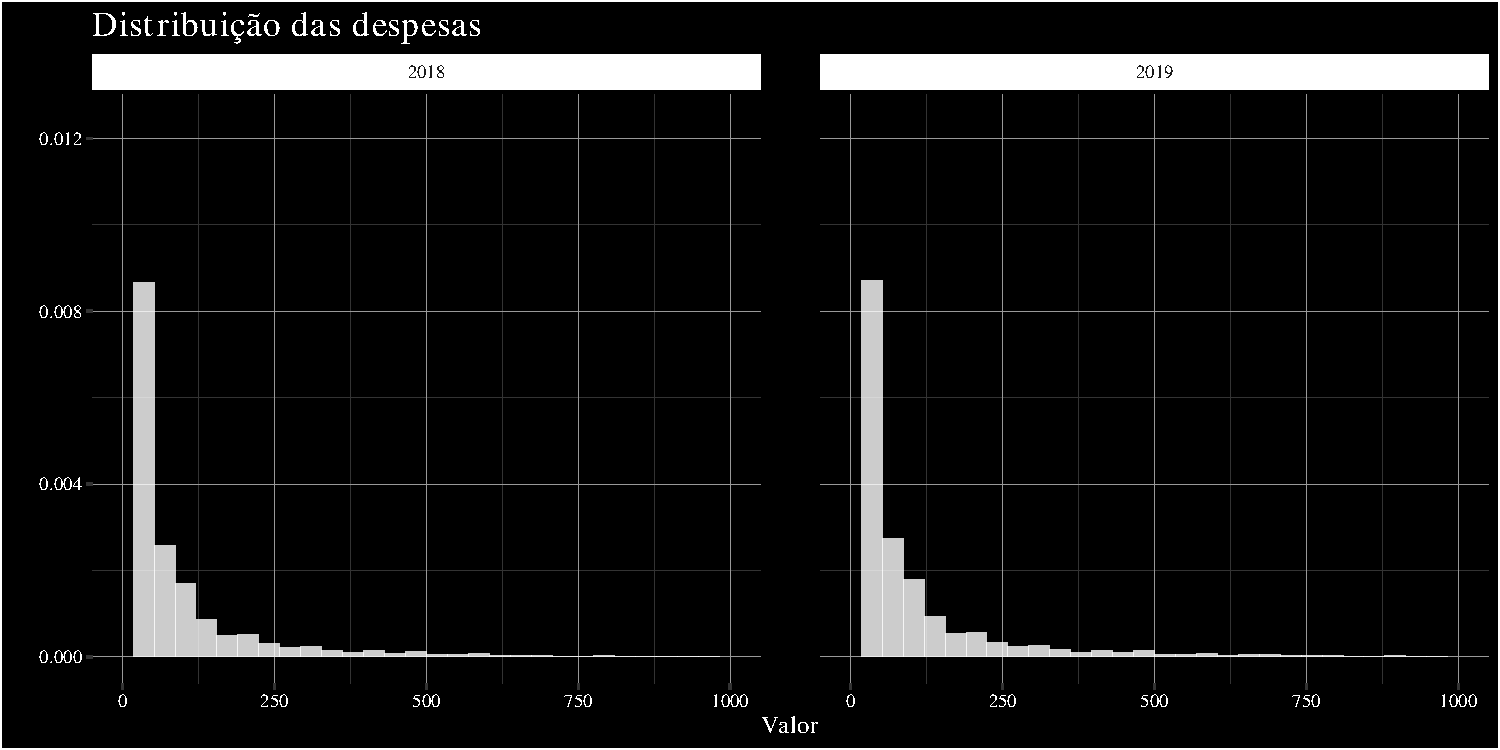
\includegraphics[width=\maxwidth]{figure/unnamed-chunk-5-1} 
\begin{kframe}\begin{alltt}
\hlcom{##histogram by month}
\hlstd{Despesas} \hlopt \hlstd{dplyr}\hlopt{::}\hlkwd{filter}\hlstd{(Valor} \hlopt{>} \hlnum{0} \hlopt{&} \hlstd{Valor} \hlopt{<} \hlnum{1000}\hlstd{)} \hlopt
    \hlkwd{ggplot}\hlstd{(}\hlkwd{aes}\hlstd{(Valor,}\hlkwc{y}\hlstd{=..density..))}\hlopt{+}
    \hlkwd{geom_histogram}\hlstd{(}\hlkwc{fill}\hlstd{=}\hlstr{"white"}\hlstd{,}\hlkwc{alpha}\hlstd{=}\hlnum{0.8}\hlstd{)}\hlopt{+}
    \hlkwd{facet_grid}\hlstd{(}\hlopt{~}\hlstd{ano )}\hlopt{+}\hlstd{temaMobills}\hlopt{+}
        \hlkwd{labs}\hlstd{(}\hlkwc{title}\hlstd{=}\hlstr{"Distribuição das despesas"}\hlstd{)}\hlopt{+}
    \hlkwd{scale_x_continuous}\hlstd{(}\hlkwc{limits}\hlstd{=}\hlkwd{c}\hlstd{(}\hlnum{0}\hlstd{,}\hlnum{1000}\hlstd{))}\hlopt{+}
  \hlkwd{facet_grid}\hlstd{(}\hlopt{~}\hlstd{mes)}
\end{alltt}


{\ttfamily\noindent\bfseries\color{errorcolor}{\#\# Error: At least one layer must contain all faceting variables: `mes`.\\\#\# * Plot is missing `mes`\\\#\# * Layer 1 is missing `mes`}}\end{kframe}
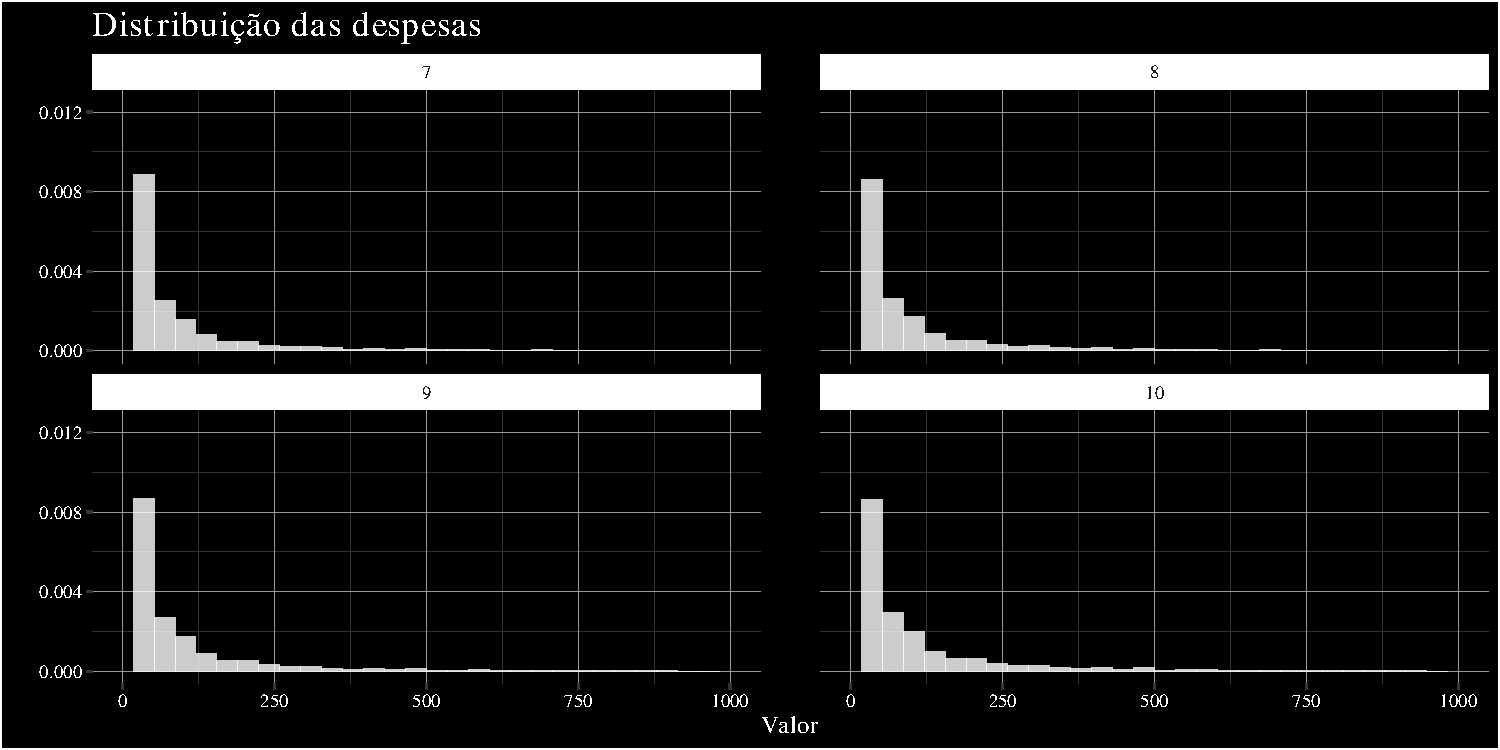
\includegraphics[width=\maxwidth]{figure/unnamed-chunk-5-2} 

\end{knitrout}


\begin{knitrout}\tiny
\definecolor{shadecolor}{rgb}{0.969, 0.969, 0.969}\color{fgcolor}\begin{kframe}
\begin{alltt}
\hlstd{desp} \hlopt
  \hlkwd{group_by}\hlstd{(mes,ano)} \hlopt
  \hlkwd{summarise}\hlstd{(}\hlkwc{contagem}\hlstd{=}\hlkwd{n}\hlstd{())} \hlopt
  \hlkwd{ggplot}\hlstd{(}\hlkwd{aes}\hlstd{(mes, contagem,}\hlkwc{labs}\hlstd{=contagem))}\hlopt{+}
  \hlkwd{geom_col}\hlstd{(}\hlkwd{aes}\hlstd{(}\hlkwc{fill}\hlstd{=contagem),}
           \hlkwc{width} \hlstd{=} \hlnum{0.5}\hlstd{)}\hlopt{+}
  \hlkwd{scale_fill_viridis}\hlstd{(}\hlkwc{option}\hlstd{=}\hlstr{"magma"}\hlstd{,}\hlkwc{begin}\hlstd{=}\hlnum{0.5}\hlstd{)}\hlopt{+}
  \hlkwd{labs}\hlstd{(}\hlkwc{title}\hlstd{=}\hlstr{"Quantidade de Despesas por mês"}\hlstd{,}
       \hlkwc{subtitle} \hlstd{=} \hlstr{"Usuarios de 16 à 24 anos, no periodo de 11 de Julho à 10 de Outubro."}\hlstd{,}
       \hlkwc{x}\hlstd{=}\hlstr{"Mês"}\hlstd{,}
       \hlkwc{y}\hlstd{=}\hlstr{"Quantidade de despesas"}\hlstd{)}\hlopt{+}
  \hlstd{temaMobills}\hlopt{+}
  \hlkwd{scale_y_continuous}\hlstd{(}\hlkwc{limits} \hlstd{=} \hlkwd{c}\hlstd{(}\hlnum{0}\hlstd{,}\hlnum{100000}\hlstd{),}
                       \hlkwc{expand}\hlstd{=}\hlkwd{c}\hlstd{(}\hlnum{0.01009}\hlstd{,}\hlnum{0.000000001}\hlstd{),}
                       \hlkwc{breaks} \hlstd{=} \hlkwd{seq}\hlstd{(}\hlnum{0}\hlstd{,}\hlnum{150000}\hlstd{,}\hlnum{10000}\hlstd{))}\hlopt{+}
  \hlkwd{geom_text}\hlstd{(}\hlkwd{aes}\hlstd{(}\hlkwc{label}\hlstd{=contagem),}
              \hlkwc{size}\hlstd{=}\hlnum{3.5}\hlstd{,}
              \hlkwc{colour}\hlstd{=}\hlstr{"white"}\hlstd{,}
              \hlkwc{vjust}\hlstd{=}\hlopt{-}\hlnum{0.2}\hlstd{)}\hlopt{+}
  \hlkwd{facet_grid}\hlstd{(}\hlopt{~}\hlstd{ano)}
\end{alltt}
\end{kframe}
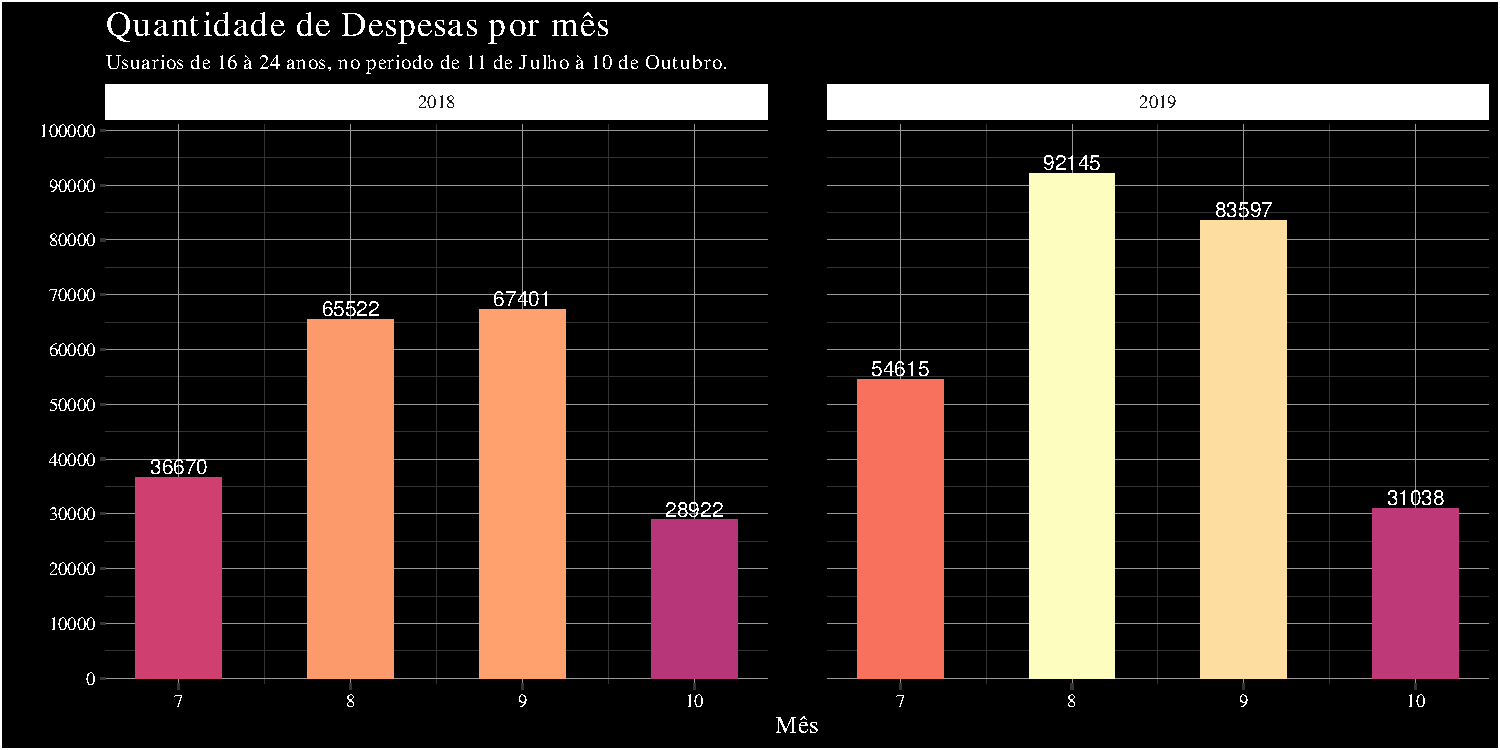
\includegraphics[width=\maxwidth]{figure/unnamed-chunk-6-1} 

\end{knitrout}


\begin{knitrout}\tiny
\definecolor{shadecolor}{rgb}{0.969, 0.969, 0.969}\color{fgcolor}\begin{kframe}
\begin{alltt}
\hlstd{Despesas} \hlopt
    \hlkwd{group_by}\hlstd{(Descricao)} \hlopt
    \hlkwd{summarise}\hlstd{(}\hlkwc{count} \hlstd{=} \hlkwd{n}\hlstd{(),} \hlkwc{valorSoma}\hlstd{=} \hlkwd{sum}\hlstd{(Valor))} \hlopt
    \hlkwd{top_n}\hlstd{(}\hlnum{100000}\hlstd{)} \hlopt \hlkwd{filter}\hlstd{(count} \hlopt{>} \hlnum{3000}\hlstd{)} \hlopt \hlkwd{arrange}\hlstd{(}\hlkwd{desc}\hlstd{(count))}\hlopt
  \hlkwd{ggplot}\hlstd{(}\hlkwd{aes}\hlstd{(}\hlkwc{x}\hlstd{=}\hlkwd{reorder}\hlstd{(Descricao,count,max),count),}\hlkwc{labels}\hlstd{=count)}\hlopt{+}\hlkwd{geom_col}\hlstd{(}\hlkwc{fill}\hlstd{=}\hlstr{"white"}\hlstd{,}\hlkwc{width} \hlstd{=} \hlnum{0.5}\hlstd{)}\hlopt{+}
  \hlkwd{coord_flip}\hlstd{()}\hlopt{+}
  \hlstd{temaMobills}\hlopt{+}
  \hlkwd{theme}\hlstd{(}\hlkwc{axis.text} \hlstd{=} \hlkwd{element_text}\hlstd{(}\hlkwc{size}\hlstd{=}\hlnum{7}\hlstd{),}
        \hlkwc{panel.grid.major.x} \hlstd{=}\hlkwd{element_line}\hlstd{(}\hlkwc{colour}\hlstd{=}\hlstr{"white"}\hlstd{,}\hlkwc{linetype} \hlstd{=} \hlnum{1}\hlstd{),}
        \hlkwc{panel.grid.minor.x} \hlstd{=} \hlkwd{element_blank}\hlstd{(),}
        \hlkwc{panel.grid.major.y} \hlstd{=} \hlkwd{element_line}\hlstd{(}\hlkwc{size}\hlstd{=}\hlnum{0.1}\hlstd{))}\hlopt{+}
  \hlkwd{geom_text}\hlstd{(}\hlkwd{aes}\hlstd{(}\hlkwc{label}\hlstd{=count),}\hlkwc{colour}\hlstd{=}\hlstr{"white"}\hlstd{,}\hlkwc{size}\hlstd{=}\hlnum{3}\hlstd{,}\hlkwc{hjust}\hlstd{=}\hlopt{-}\hlnum{0.5}\hlstd{)}\hlopt{+}
  \hlkwd{scale_y_continuous}\hlstd{(}\hlkwc{limits}\hlstd{=}\hlkwd{c}\hlstd{(}\hlnum{0}\hlstd{,}\hlnum{32000}\hlstd{))}
\end{alltt}
\end{kframe}
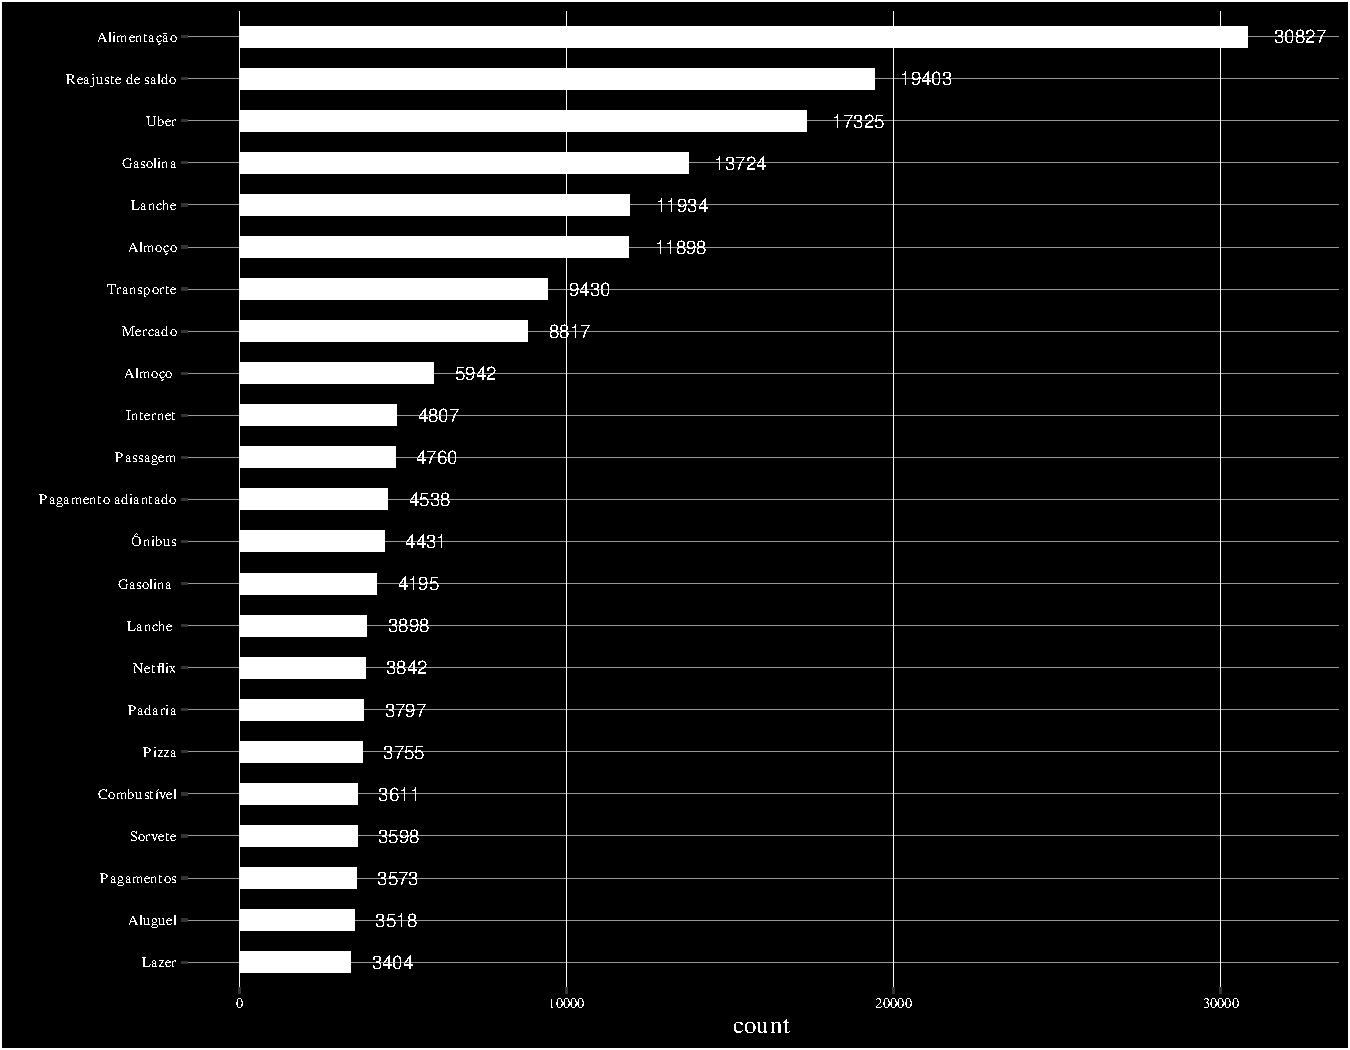
\includegraphics[width=\maxwidth]{figure/unnamed-chunk-7-1} 

\end{knitrout}

\begin{knitrout}\tiny
\definecolor{shadecolor}{rgb}{0.969, 0.969, 0.969}\color{fgcolor}\begin{kframe}
\begin{alltt}
\hlstd{Despesas} \hlopt
    \hlkwd{group_by}\hlstd{(Descricao)} \hlopt
    \hlkwd{summarise}\hlstd{(}\hlkwc{count} \hlstd{=} \hlkwd{n}\hlstd{(),} \hlkwc{valorSoma}\hlstd{=} \hlkwd{sum}\hlstd{(Valor))} \hlopt
    \hlkwd{top_n}\hlstd{(}\hlnum{100000}\hlstd{)} \hlopt \hlkwd{filter}\hlstd{(count} \hlopt{<}\hlnum{3000}\hlstd{,count}\hlopt{>}\hlnum{1500}\hlstd{)} \hlopt \hlkwd{arrange}\hlstd{(}\hlkwd{desc}\hlstd{(count))}\hlopt
  \hlkwd{ggplot}\hlstd{(}\hlkwd{aes}\hlstd{(}\hlkwc{x}\hlstd{=}\hlkwd{reorder}\hlstd{(Descricao,count,max),count),}\hlkwc{labels}\hlstd{=count)}\hlopt{+}\hlkwd{geom_col}\hlstd{(}\hlkwc{fill}\hlstd{=}\hlstr{"white"}\hlstd{,}\hlkwc{width} \hlstd{=} \hlnum{0.5}\hlstd{)}\hlopt{+}
  \hlkwd{coord_flip}\hlstd{()}\hlopt{+}
  \hlstd{temaMobills}\hlopt{+}
  \hlkwd{theme}\hlstd{(}\hlkwc{axis.text} \hlstd{=} \hlkwd{element_text}\hlstd{(}\hlkwc{size}\hlstd{=}\hlnum{7}\hlstd{),}
        \hlkwc{panel.grid.major.x} \hlstd{=}\hlkwd{element_line}\hlstd{(}\hlkwc{colour}\hlstd{=}\hlstr{"white"}\hlstd{,}\hlkwc{linetype} \hlstd{=} \hlnum{1}\hlstd{),}
        \hlkwc{panel.grid.minor.x} \hlstd{=} \hlkwd{element_blank}\hlstd{(),}
        \hlkwc{panel.grid.major.y} \hlstd{=} \hlkwd{element_line}\hlstd{(}\hlkwc{size}\hlstd{=}\hlnum{0.1}\hlstd{))}\hlopt{+}
  \hlkwd{geom_text}\hlstd{(}\hlkwd{aes}\hlstd{(}\hlkwc{label}\hlstd{=count),}\hlkwc{colour}\hlstd{=}\hlstr{"white"}\hlstd{,}\hlkwc{size}\hlstd{=}\hlnum{3}\hlstd{,}\hlkwc{hjust}\hlstd{=}\hlopt{-}\hlnum{0.5}\hlstd{)}\hlopt{+}
  \hlkwd{scale_y_continuous}\hlstd{(}\hlkwc{limits}\hlstd{=}\hlkwd{c}\hlstd{(}\hlnum{0}\hlstd{,}\hlnum{32000}\hlstd{))}
\end{alltt}
\end{kframe}
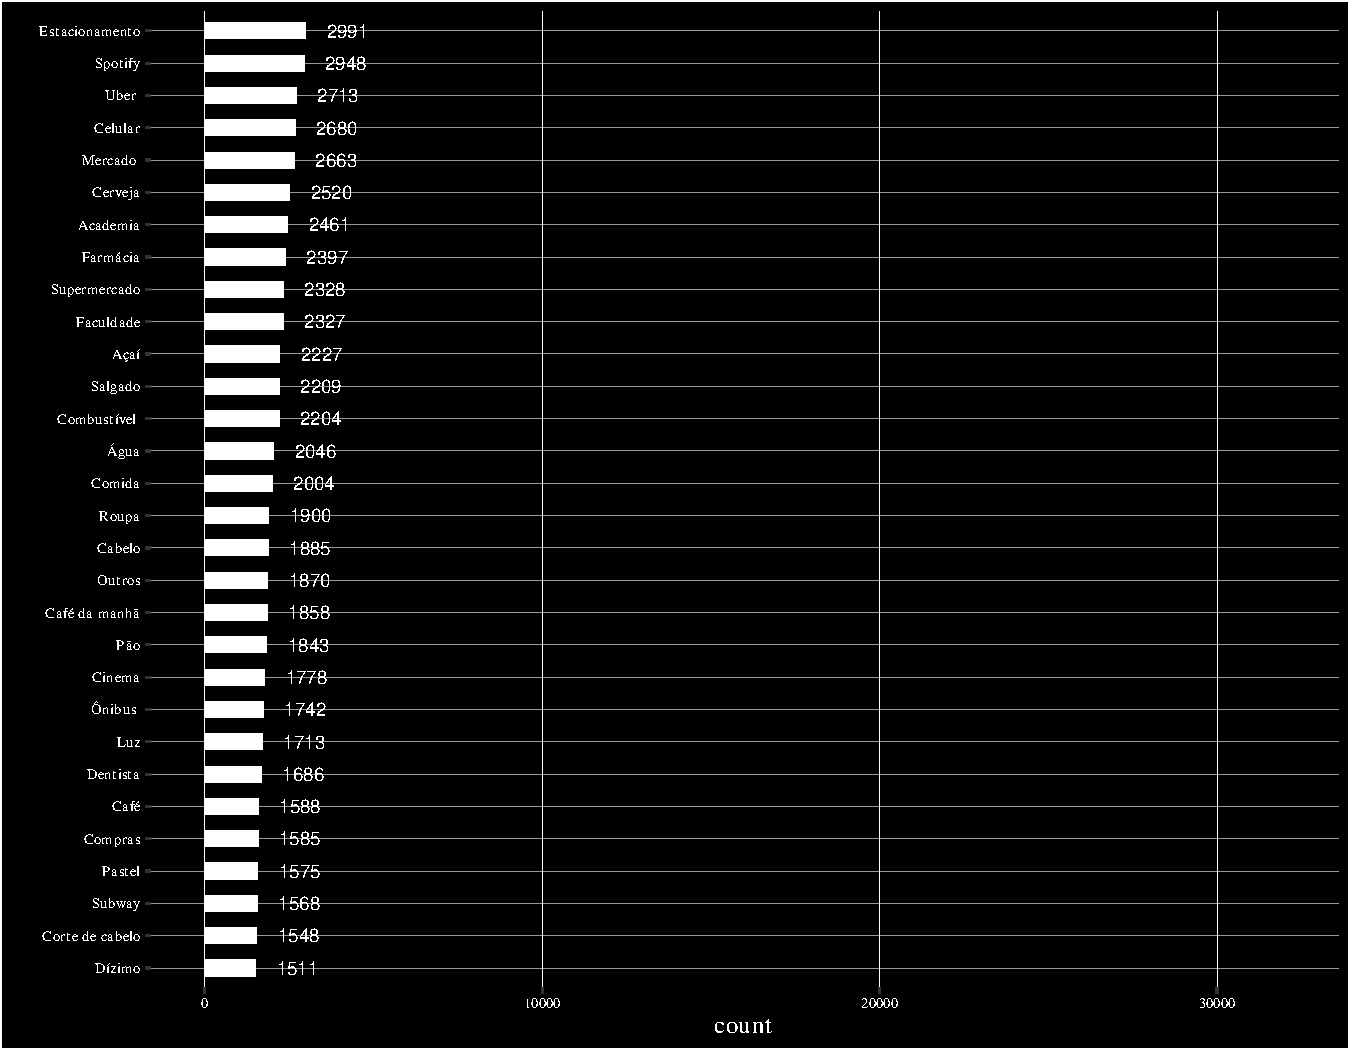
\includegraphics[width=\maxwidth]{figure/unnamed-chunk-8-1} 

\end{knitrout}


\end{document}
